% TikZ plot for 2025_yolo_2023
% Generated automatically with embedded data
% Requires: \usepackage{pgfplots} \pgfplotsset{compat=1.18}

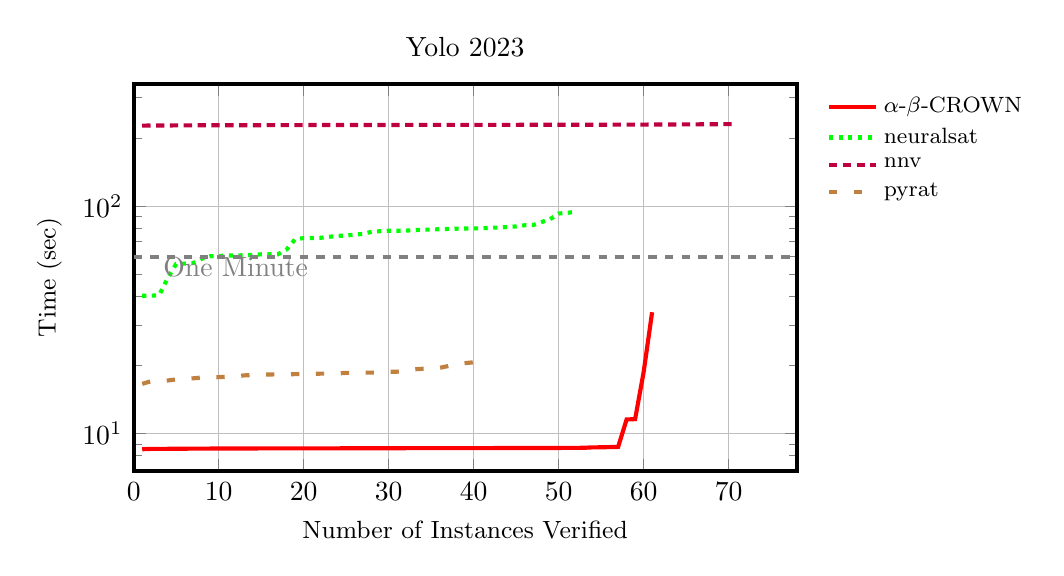
\begin{tikzpicture}
\begin{semilogyaxis}[
    xlabel={Number of Instances Verified},
    ylabel={Time (sec)},
    legend pos=outer north east,
    grid=major,
    width=10cm,
    height=6.5cm,
    ymin=6.826,
    ymax=344.8,
    xmin=0,
    xmax=78,
    line width=1.5pt,
    legend style={font=\footnotesize, cells={anchor=west}, draw=none},
    xlabel style={font=\small},
    ylabel style={font=\small},
    title={Yolo 2023},
    title style={font=\normalsize}
]

\addplot[color=red, mark=none, solid] coordinates {
    (1,8.532145)
    (2,8.561727)
    (3,8.563659)
    (4,8.568970)
    (5,8.574114)
    (6,8.580673)
    (7,8.584019)
    (8,8.589070)
    (9,8.590281)
    (10,8.595801)
    (11,8.597310)
    (12,8.602728)
    (13,8.602926)
    (14,8.603275)
    (15,8.603781)
    (16,8.604016)
    (17,8.604136)
    (18,8.606345)
    (19,8.607530)
    (20,8.608353)
    (21,8.609177)
    (22,8.609181)
    (23,8.610919)
    (24,8.611793)
    (25,8.613373)
    (26,8.613739)
    (27,8.617323)
    (28,8.620409)
    (29,8.621172)
    (30,8.622199)
    (31,8.624003)
    (32,8.625124)
    (33,8.627635)
    (34,8.627733)
    (35,8.627846)
    (36,8.628078)
    (37,8.628481)
    (38,8.629450)
    (39,8.630684)
    (40,8.631340)
    (41,8.632472)
    (42,8.632564)
    (43,8.636615)
    (44,8.637333)
    (45,8.638575)
    (46,8.642158)
    (47,8.642253)
    (48,8.643891)
    (49,8.644079)
    (50,8.644623)
    (51,8.653412)
    (52,8.653958)
    (53,8.657470)
    (54,8.698330)
    (55,8.701085)
    (56,8.721793)
    (57,8.735547)
    (58,11.536478)
    (59,11.575146)
    (60,18.615767)
    (61,34.177662)
};
\addlegendentry{$\alpha$-$\beta$-CROWN}

\addplot[color=green, mark=none, dotted] coordinates {
    (1,40.361226)
    (2,40.386124)
    (3,40.650371)
    (4,48.325297)
    (5,55.750318)
    (6,55.912860)
    (7,56.262886)
    (8,58.772616)
    (9,60.282146)
    (10,60.437274)
    (11,60.676200)
    (12,60.680668)
    (13,60.910507)
    (14,61.049508)
    (15,61.440427)
    (16,61.455521)
    (17,61.522255)
    (18,64.557176)
    (19,71.630965)
    (20,72.408143)
    (21,72.459747)
    (22,72.642976)
    (23,73.379622)
    (24,74.027188)
    (25,74.312878)
    (26,75.013321)
    (27,75.558860)
    (28,77.240408)
    (29,77.642692)
    (30,77.996450)
    (31,78.013808)
    (32,78.097719)
    (33,78.577806)
    (34,78.820426)
    (35,78.952247)
    (36,79.252411)
    (37,79.482827)
    (38,79.653683)
    (39,79.832568)
    (40,79.867747)
    (41,79.958915)
    (42,80.453713)
    (43,80.569791)
    (44,81.027139)
    (45,81.488299)
    (46,82.455734)
    (47,82.644911)
    (48,85.183347)
    (49,87.720396)
    (50,92.864262)
    (51,93.514187)
    (52,94.500401)
};
\addlegendentry{neuralsat}

\addplot[color=purple, mark=none, densely dashed] coordinates {
    (1,226.174988)
    (2,226.469930)
    (3,226.539315)
    (4,226.575109)
    (5,226.745540)
    (6,226.778804)
    (7,226.884842)
    (8,226.966521)
    (9,227.015979)
    (10,227.035360)
    (11,227.037189)
    (12,227.059454)
    (13,227.152172)
    (14,227.225545)
    (15,227.233862)
    (16,227.286502)
    (17,227.355448)
    (18,227.413385)
    (19,227.419786)
    (20,227.484690)
    (21,227.544186)
    (22,227.588023)
    (23,227.616007)
    (24,227.632495)
    (25,227.646365)
    (26,227.690147)
    (27,227.720100)
    (28,227.738040)
    (29,227.769634)
    (30,227.774097)
    (31,227.799915)
    (32,227.831612)
    (33,227.866050)
    (34,227.869510)
    (35,227.869530)
    (36,227.879338)
    (37,227.892394)
    (38,227.917364)
    (39,227.919534)
    (40,227.922109)
    (41,227.967972)
    (42,227.968480)
    (43,228.007245)
    (44,228.024257)
    (45,228.036970)
    (46,228.076057)
    (47,228.171986)
    (48,228.177916)
    (49,228.198636)
    (50,228.200719)
    (51,228.234493)
    (52,228.241493)
    (53,228.313524)
    (54,228.318976)
    (55,228.323924)
    (56,228.402271)
    (57,228.408166)
    (58,228.413093)
    (59,228.474276)
    (60,228.582233)
    (61,228.684699)
    (62,228.789235)
    (63,228.867512)
    (64,229.001226)
    (65,229.053340)
    (66,229.113953)
    (67,229.286151)
    (68,229.471512)
    (69,229.579685)
    (70,229.713269)
    (71,229.853390)
};
\addlegendentry{nnv}

\addplot[color=brown, mark=none, loosely dashed] coordinates {
    (1,16.545238)
    (2,16.980536)
    (3,17.003449)
    (4,17.121992)
    (5,17.303009)
    (6,17.396743)
    (7,17.499204)
    (8,17.634996)
    (9,17.649586)
    (10,17.715170)
    (11,17.780093)
    (12,17.827010)
    (13,18.033584)
    (14,18.082945)
    (15,18.192584)
    (16,18.200507)
    (17,18.212590)
    (18,18.217426)
    (19,18.259489)
    (20,18.299526)
    (21,18.318325)
    (22,18.347139)
    (23,18.369135)
    (24,18.386534)
    (25,18.492033)
    (26,18.511403)
    (27,18.539815)
    (28,18.547196)
    (29,18.554031)
    (30,18.698925)
    (31,18.718534)
    (32,18.894237)
    (33,19.174138)
    (34,19.276354)
    (35,19.303262)
    (36,19.461373)
    (37,19.818661)
    (38,20.301534)
    (39,20.407435)
    (40,20.586760)
};
\addlegendentry{pyrat}

% Timeout line
\addplot[color=gray, dashed, mark=none, domain=0:78] {60};

% Add timeout label as text below the line
\node[color=gray] at (axis cs:12,54.0) {One Minute};

\end{semilogyaxis}
\end{tikzpicture}
